\subsection{Retrospective Volatility-Model Assessment}
\label{sec:forecasting}

The preceding analyses identify cross-sectional dependency structure in B3 equities. We now ask whether adding structural descriptors improves realized-volatility forecast accuracy. The RMT and network descriptors are estimated from the full synchronized sample, so this is a retrospective comparison rather than a point-in-time forecasting design.

The chronological test period is 2021--2025. Specifications are selected by mean validation QLIKE within each model family and feature set; no test-period metric is used for selection. Figure~\ref{fig:forecast_comparison} shows aggregated test QLIKE. Lower values indicate lower loss. The confidence intervals are circular moving-block bootstrap intervals and are descriptive; paired HAC tests provide the focused feature-set comparisons below.

\begin{center}
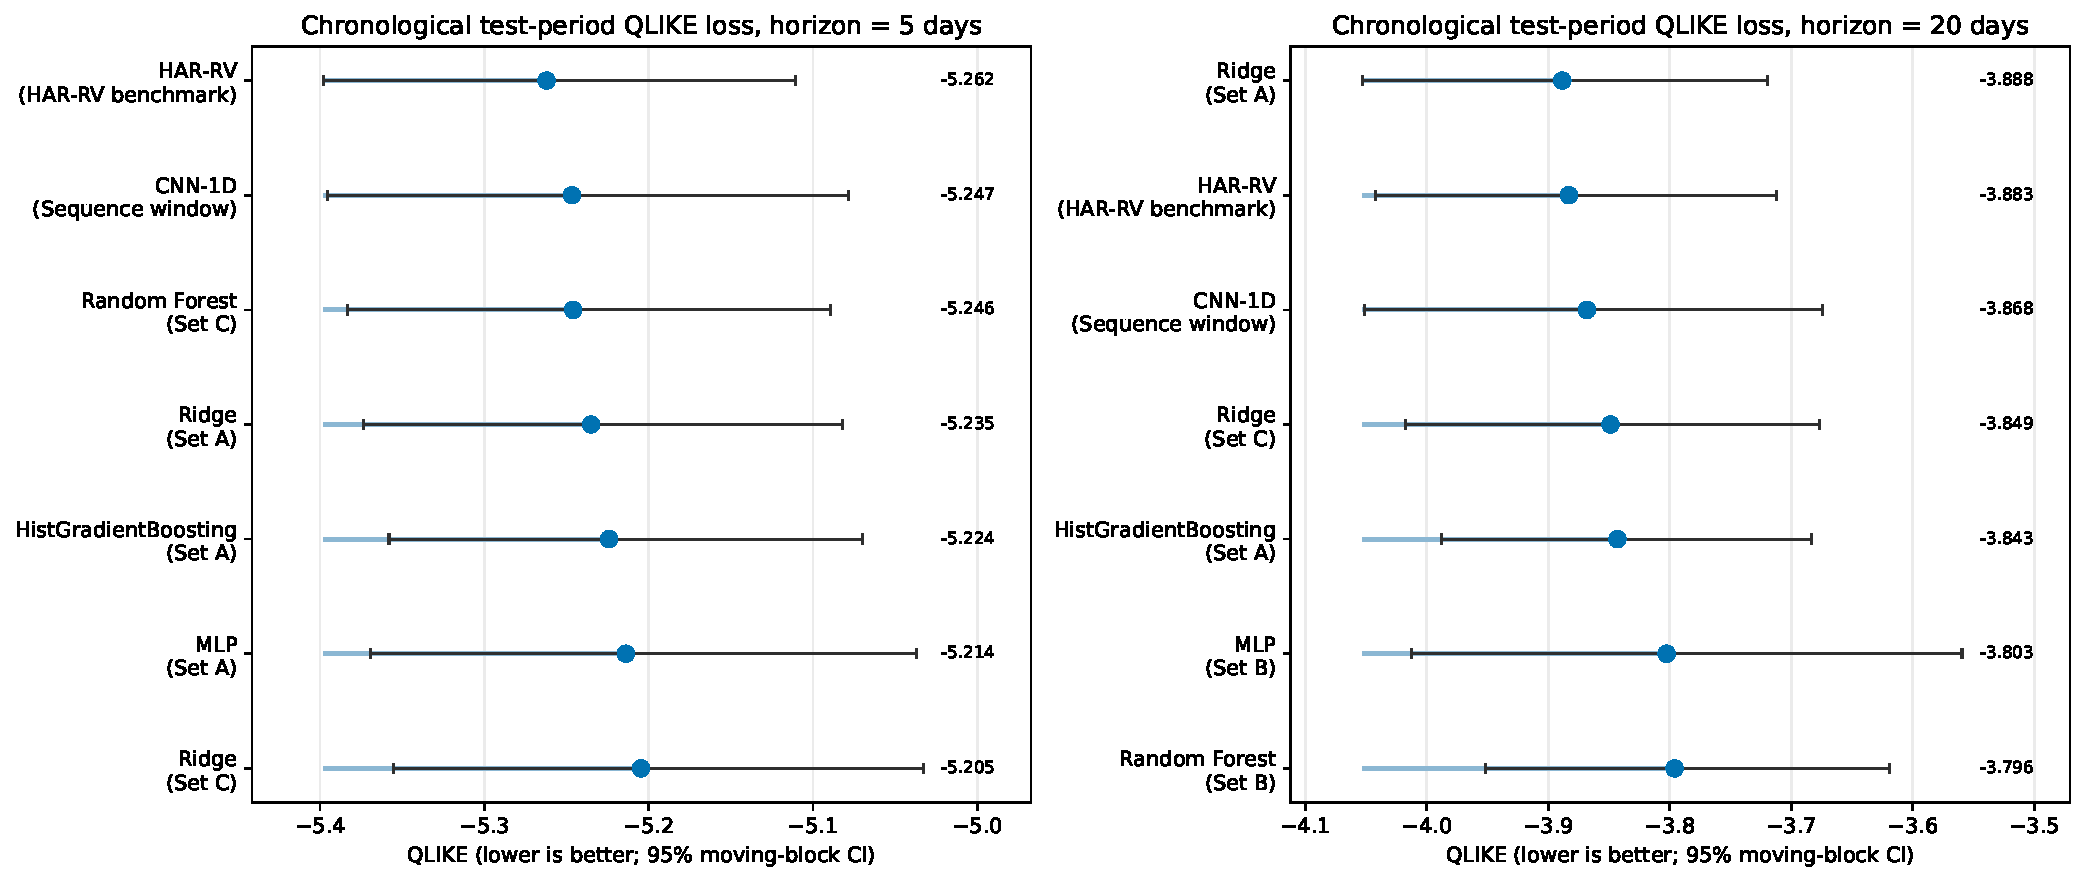
\includegraphics[width=\linewidth,height=0.58\textheight,keepaspectratio]{images/figure_16_volatility_forecast_model_comparison.pdf}
\captionof{figure}{Chronological test-period QLIKE across validation-selected specifications. Points show the mean across PETR4, VALE3 and BBDC4; bars show 95\% circular moving-block bootstrap intervals from 2,000 replications, with block length equal to the forecast horizon.}
\label{fig:forecast_comparison}
\end{center}

HAR-RV has the lowest mean QLIKE at the 5-day horizon; at 20 days, the explicit Ridge Set A comparator has a slightly lower mean than HAR-RV. The bootstrap intervals overlap substantially, so these descriptive rankings do not establish that either specification is significantly better than every alternative. The primary structural comparison is between validation-selected Ridge Set A and Ridge Set B/C, because these specifications isolate the addition of market/RMT and network descriptors while keeping the model family fixed.

Table~\ref{tab:forecast_comparison} gives validation-selected test summaries, the explicit Ridge Set A comparator, and HAR-RV. The asset-level results, block-length sensitivity and five-seed neural sensitivity are reported in Tables~\ref{tab:app_forecast},~\ref{tab:app_blocks} and~\ref{tab:app_seeds}.

\begin{center}
\captionof{table}{Validation-selected model results and the fixed Ridge Set A comparator on the 2021--2025 test period. Metrics are averaged across PETR4, VALE3 and BBDC4.}
\label{tab:forecast_comparison}
\resizebox{\linewidth}{!}{%
\begin{tabular}{lllrrrrr}
\toprule
Horizon & Model & Feature set & MAE & RMSE & QLIKE & 95\% CI for QLIKE & $R^2_{\mathrm{oos}}$ \\
\midrule
5 & CNN-1D & Sequence window & 0.0145 & 0.0213 & $-5.2467$ & $[-5.3955, -5.0784]$ & 0.2871 \\
5 & Random Forest & Set C (+Network) & 0.0162 & 0.0227 & $-5.2460$ & $[-5.3834, -5.0895]$ & 0.2001 \\
5 & HistGradientBoosting & Set A (Classical) & 0.0168 & 0.0235 & $-5.2241$ & $[-5.3581, -5.0700]$ & 0.1468 \\
5 & MLP & Set A (Classical) & 0.0138 & 0.0209 & $-5.2139$ & $[-5.3692, -5.0369]$ & 0.3150 \\
5 & Ridge & Set C (+Network) & 0.0146 & 0.0215 & $-5.2047$ & $[-5.3553, -5.0329]$ & 0.2733 \\
20 & CNN-1D & Sequence window & 0.0210 & 0.0308 & $-3.8682$ & $[-4.0509, -3.6740]$ & 0.3947 \\
20 & Ridge & Set C (+Network) & 0.0224 & 0.0316 & $-3.8487$ & $[-4.0177, -3.6765]$ & 0.3587 \\
20 & HistGradientBoosting & Set A (Classical) & 0.0265 & 0.0375 & $-3.8430$ & $[-3.9879, -3.6834]$ & 0.1560 \\
20 & MLP & Set B (+Market/RMT) & 0.0220 & 0.0322 & $-3.8026$ & $[-4.0126, -3.5595]$ & 0.3514 \\
20 & Random Forest & Set B (+Market/RMT) & 0.0284 & 0.0405 & $-3.7960$ & $[-3.9514, -3.6195]$ & 0.0124 \\
5 & Ridge (Set A baseline) & Set A (Classical) & 0.0146 & 0.0213 & $-5.2351$ & $[-5.3736, -5.0820]$ & 0.2813 \\
5 & HAR-RV & HAR-RV benchmark & 0.0157 & 0.0222 & $-5.2622$ & $[-5.3978, -5.1109]$ & 0.2228 \\
20 & Ridge (Set A baseline) & Set A (Classical) & 0.0217 & 0.0306 & $-3.8884$ & $[-4.0528, -3.7198]$ & 0.3941 \\
20 & HAR-RV & HAR-RV benchmark & 0.0240 & 0.0335 & $-3.8830$ & $[-4.0422, -3.7123]$ & 0.2826 \\
\bottomrule
\end{tabular}}
\end{center}

\noindent\footnotesize\emph{Notes:} QLIKE is defined in Eq.~\eqref{eq:theory_qlike}; $R^2_{\mathrm{oos}}$ is relative to the training-sample mean benchmark. Set A contains point-in-time return and volatility predictors; Set B adds market and full-sample RMT descriptors; Set C additionally includes full-sample MST and PMFG descriptors. Sets B and C are retrospective structural specifications.
\normalsize

We compare validation-selected Ridge Set B/C with Ridge Set A using date-level mean QLIKE differences across the three assets and Newey--West standard errors with horizon-specific lags. The same test also reports HAR-RV versus Ridge Set A. The difference is defined as baseline QLIKE minus candidate QLIKE, so a positive value favours the candidate. Table~\ref{tab:forecast_loss_test} reports two-sided $p$-values; Holm adjustment is applied across the four structural contrasts.

\begin{center}
\captionof{table}{HAC tests of validation-selected feature-set contrasts and HAR-RV against Ridge Set A. Negative differences favour the Set A baseline.}
\label{tab:forecast_loss_test}
\resizebox{\linewidth}{!}{%
\begin{tabular}{rlrrrrrr}
\toprule
Horizon & Contrast & Mean difference & HAC s.e. & Statistic & Two-sided $p$ & Holm $p$ \\
\midrule
5 & Set B vs Set A & -0.023021 & 0.006010 & -3.831 & 0.000128 & 0.000384 \\
5 & Set C vs Set A & -0.030401 & 0.007332 & -4.147 & 0.000034 & 0.000135 \\
20 & Set B vs Set A & -0.029578 & 0.010914 & -2.710 & 0.006727 & 0.006727 \\
20 & Set C vs Set A & -0.039761 & 0.011464 & -3.468 & 0.000524 & 0.001047 \\
5 & HAR-RV vs Ridge A & -0.027097 & 0.015080 & -1.797 & 0.072348 & -- \\
20 & HAR-RV vs Ridge A & 0.005454 & 0.011444 & 0.477 & 0.633657 & -- \\
\bottomrule
\end{tabular}}
\end{center}

\noindent\footnotesize\emph{Notes:} The loss difference is QLIKE$_{\mathrm{Ridge\ A}}-$QLIKE$_{\mathrm{candidate}}$, averaged by date across the three assets. Newey--West lags are 4 and 19 for the 5- and 20-day horizons. Holm adjustment covers the four Set B/C versus Set A tests; HAR-RV contrasts are shown separately and are not included in that family.
\normalsize

All four Ridge Set B/C contrasts have negative mean differences, and their two-sided HAC tests remain significant after Holm adjustment. Thus, in this retrospective test, adding the structural feature sets does not improve QLIKE over Ridge Set A; the observed losses are higher. The HAR-RV versus Ridge Set A comparison is not significant at either horizon. These results answer the accuracy question for the evaluated pooled assets and split, but do not establish performance for recursively estimated, point-in-time structural features.

\begin{center}
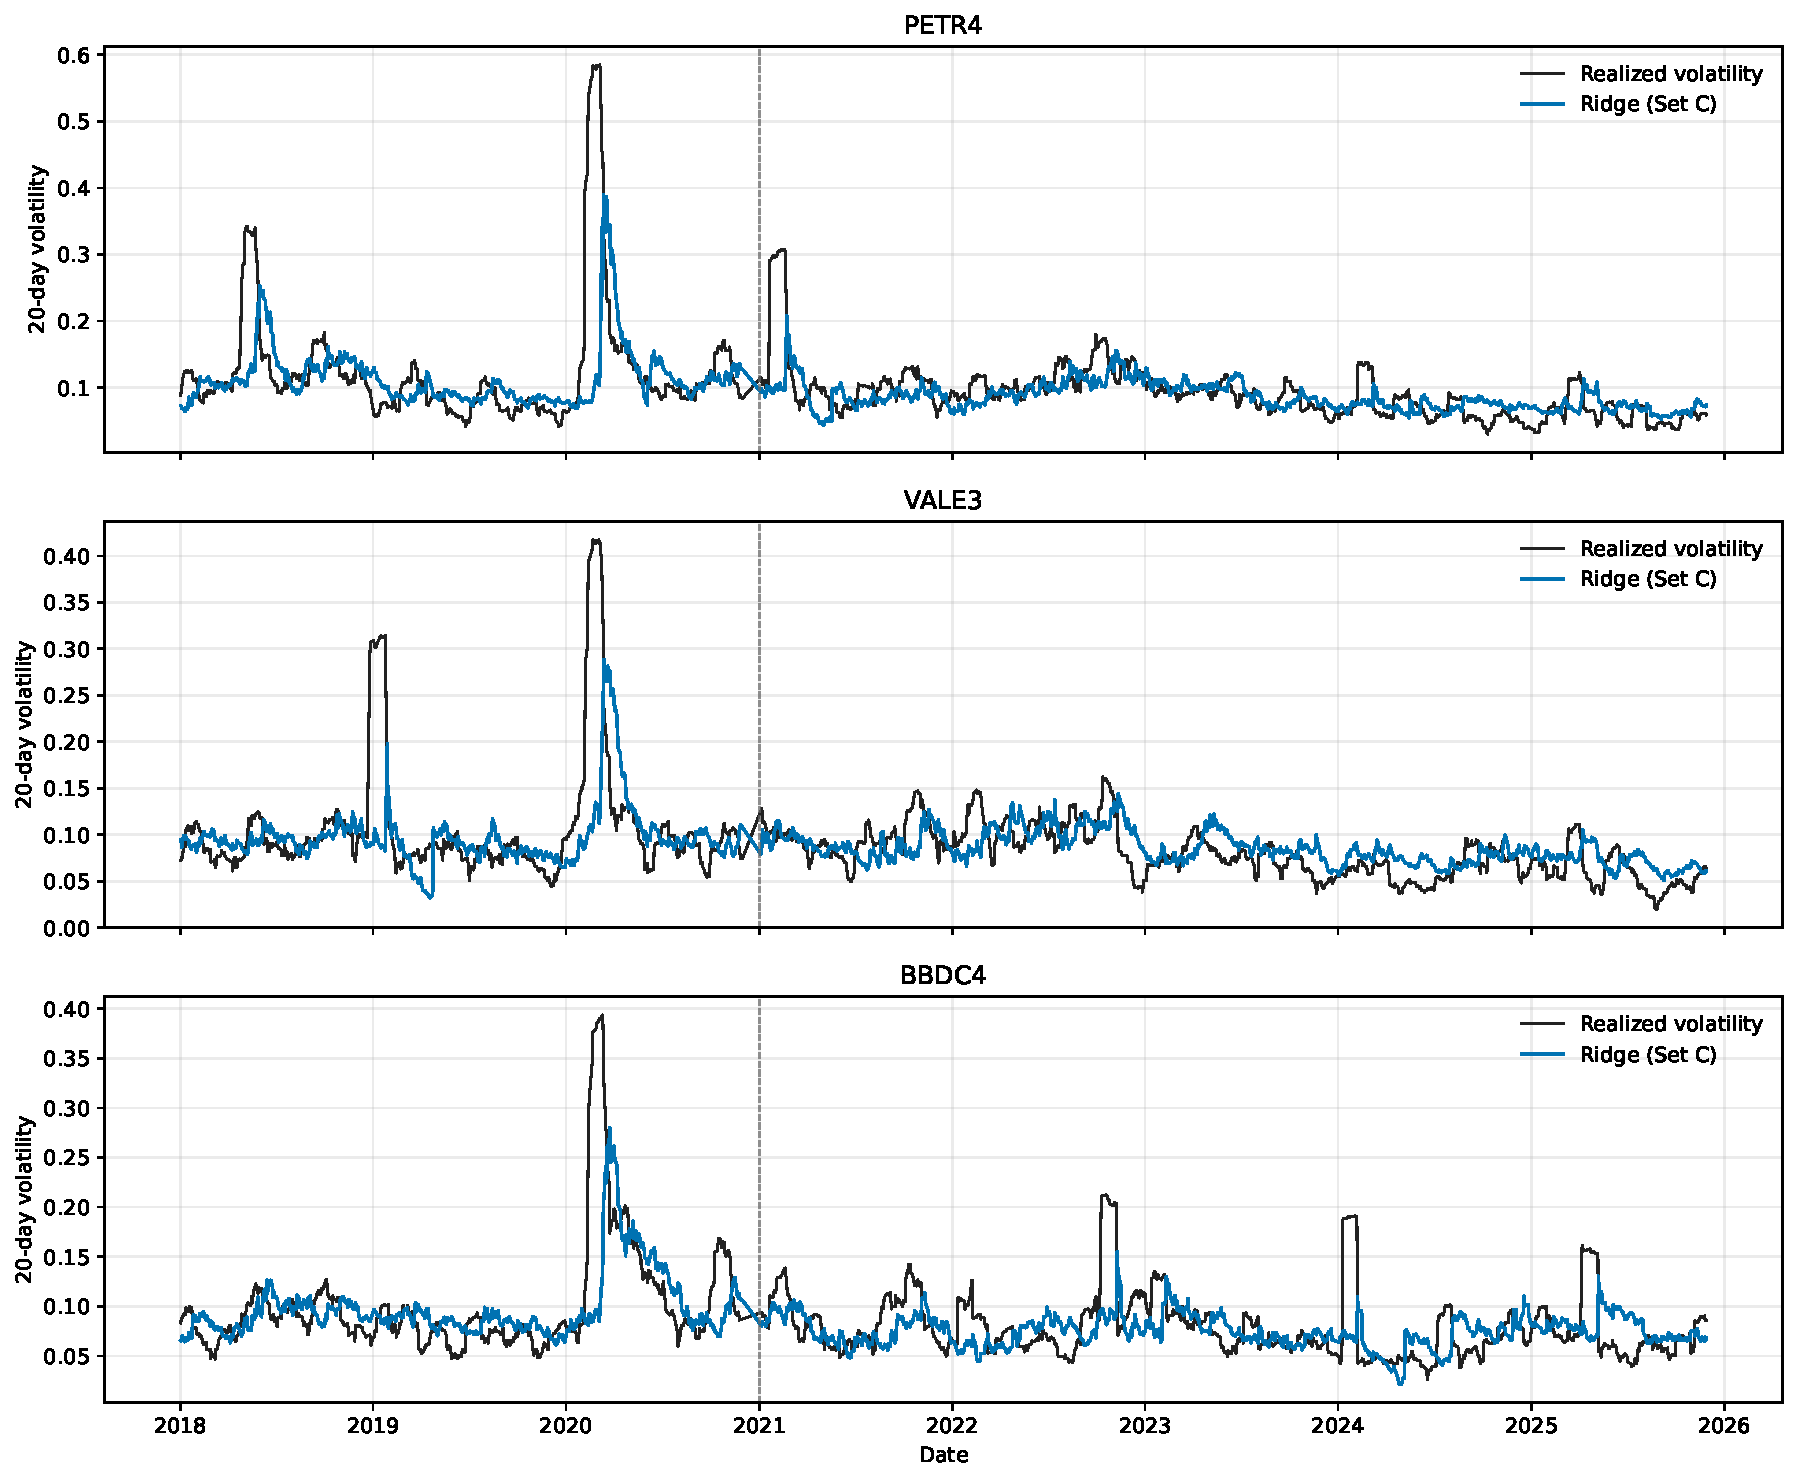
\includegraphics[width=0.95\linewidth,height=0.58\textheight,keepaspectratio]{images/figure_17_realized_vs_predicted_volatility.pdf}
\captionof{figure}{Realized and predicted 20-day volatility for PETR4, VALE3 and BBDC4 using the specification selected on validation data. The vertical dashed line marks the beginning of the 2021--2025 test period.}
\label{fig:realized_vs_predicted}
\end{center}

Figure~\ref{fig:realized_vs_predicted} shows that forecasts follow persistent volatility changes but smooth abrupt realized spikes and subsequent reversals. This visual pattern complements, but does not replace, the aggregate loss comparisons.

Figure~\ref{fig:feature_importance} reports the largest Random Forest impurity-based importance entries across candidate feature sets at each horizon. These values describe how fitted trees use predictors; they do not estimate marginal forecast gains or causal contributions.

\begin{center}
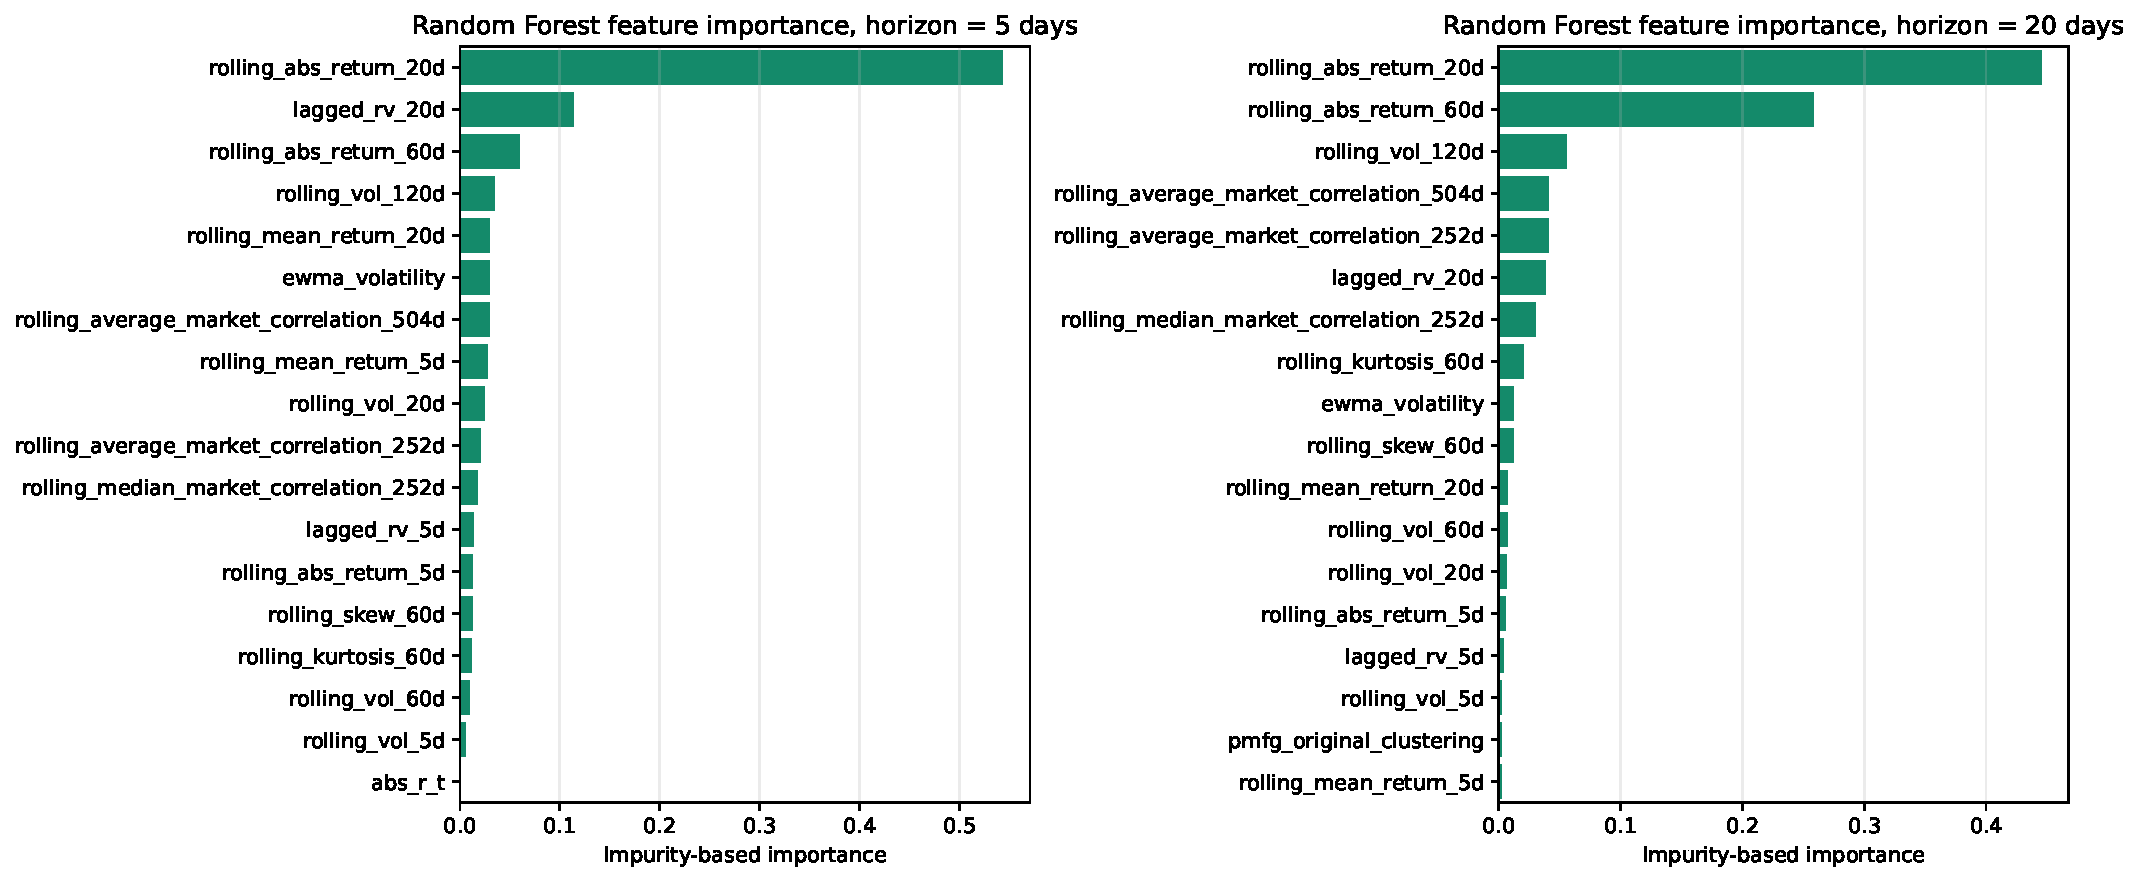
\includegraphics[width=0.95\linewidth,height=0.58\textheight,keepaspectratio]{images/figure_18_ml_feature_importance.pdf}
\captionof{figure}{Random Forest impurity-based importance for the validation-selected feature set at each horizon. Importance is descriptive and is not a measure of incremental predictive value.}
\label{fig:feature_importance}
\end{center}

Conventional volatility predictors account for most of the highest-ranked entries. Structural descriptors also appear in selected models, but their presence among tree splits does not override the test result: the paired Ridge comparisons do not show an accuracy gain from Set B or Set C. Neural-seed sensitivity and block-length sensitivity are documented in Tables~\ref{tab:app_seeds} and~\ref{tab:app_blocks}.
